\section{Lösungsidee}
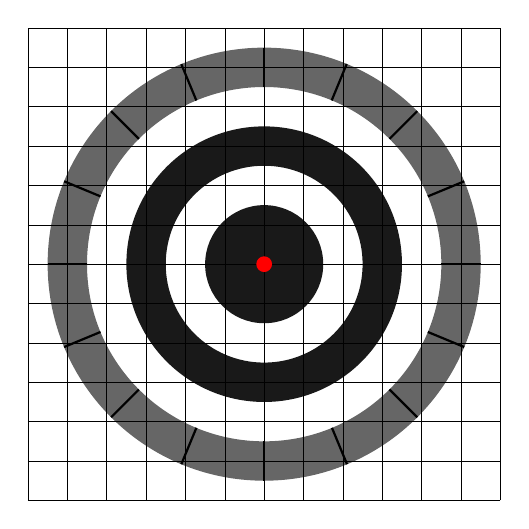
\begin{tikzpicture}[scale=0.5]
	\fill[black!90!white] (0,0) circle [radius=1.5];
	\fill[black!90!white, even odd rule] (0,0) circle[radius=2.5] circle[radius=3.5];
	\fill[black!60!white, even odd rule] (0,0) circle[radius=4.5] circle[radius=5.5];

	\foreach \angle in {0, 22.5, 45, 67.590, 90, 112.5, 135, 157.5, 180, 202.5, 225, 247.5, 270, 292.5, 315, 337.5} 
    	\draw[thick] (\angle:4.5) -- (\angle:5.5);

	\draw[very thin] (-6, -6) grid (6, 6);
	\fill[red] (0,0) circle[radius=0.2];
\end{tikzpicture}

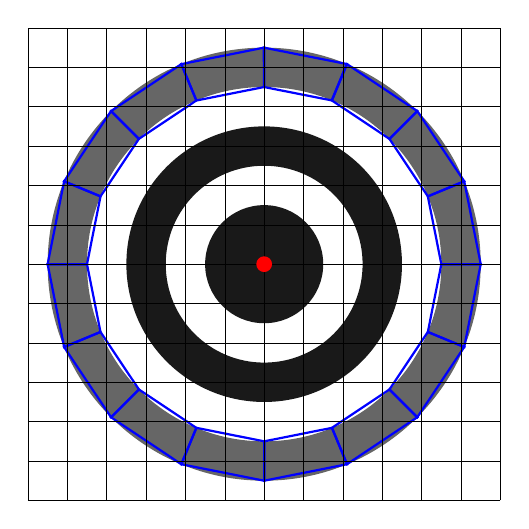
\begin{tikzpicture}[scale=0.5]
	\fill[black!90!white] (0,0) circle [radius=1.5];
	\fill[black!90!white, even odd rule] (0,0) circle[radius=2.5] circle[radius=3.5];
	\fill[black!60!white, even odd rule] (0,0) circle[radius=4.5] circle[radius=5.5];

	\foreach \angle in {0, 22.5, 45, 67.590, 90, 112.5, 135, 157.5, 180, 202.5, 225, 247.5, 270, 292.5, 315, 337.5} 
    	\draw[blue, thick] (\angle:4.5) -- (\angle:5.5) -- (\angle+22.5:5.5) -- (\angle+22.5:4.5) -- cycle;

	\draw[very thin] (-6, -6) grid (6, 6);
	\fill[red] (0,0) circle[radius=0.2];
\end{tikzpicture}

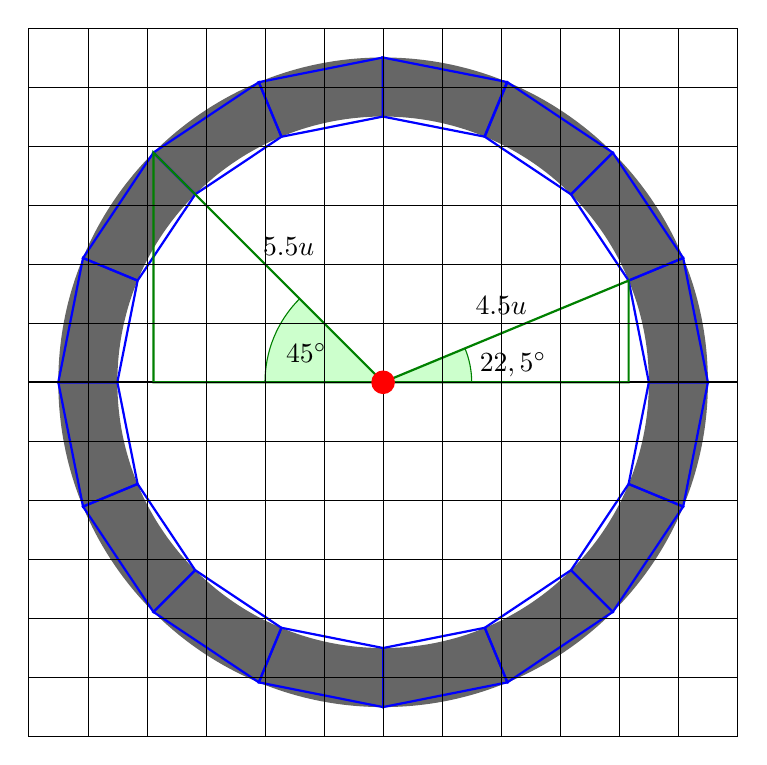
\begin{tikzpicture}[scale=0.75]
	\fill[black!60!white, even odd rule] (0,0) circle[radius=4.5] circle[radius=5.5];

	\foreach \angle in {0, 22.5, 45, 67.590, 90, 112.5, 135, 157.5, 180, 202.5, 225, 247.5, 270, 292.5, 315, 337.5} 
    	\draw[blue, thick] (\angle:4.5) -- (\angle:5.5) -- (\angle+22.5:5.5) -- (\angle+22.5:4.5) -- cycle;

	\draw[thick] (-6,0) -- (6,0);

	\filldraw[fill=green!20,draw=green!50!black] (0,0) -- (1.5,0) arc[start angle=0, end angle=22.5, radius=1.5];
	\draw[green!50!black, thick] (0,0) -- (22.5:4.5) -- (22.5:4.5 |- 0,0) -- (0,0);

	\draw (2, 1.3) node {\(4.5u\)};
	\draw (2.2, 0.3) node {\(22,5^{\circ}\)};

	\filldraw[fill=green!20,draw=green!50!black] (0,0) -- (-2,0) arc[start angle=180, end angle=135, radius=2];
	\draw[green!50!black, thick] (0,0) -- (135:5.5) -- (135:5.5 |- 0,0) -- (0,0);

	\draw (-1.6, 2.3) node {\(5.5u\)};
	\draw (-1.3, 0.5) node {\(45^{\circ}\)};

	\draw[very thin] (-6, -6) grid (6, 6);
	\fill[red] (0,0) circle[radius=0.2];
\end{tikzpicture}

\begin{align}
\begin{split}
\text{Innerer Ring:} \\
x = cos(w) * 4,5 \\
y = sin(w) * 4,5
\end{split}
\begin{split}
\text{Äußerer Ring:} \\
x = cos(w) * 5,5 \\
y = sin(w) * 5,5
\end{split}
\end{align}

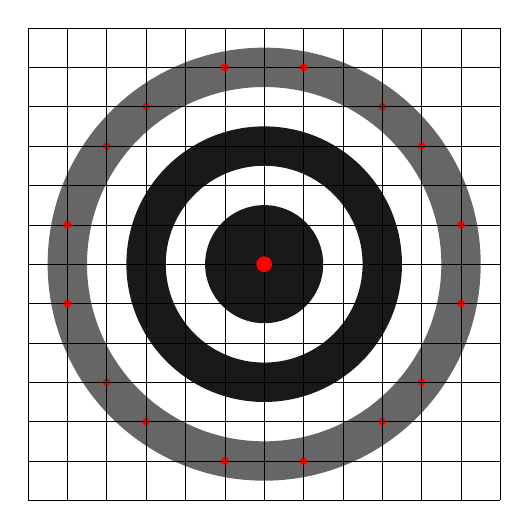
\begin{tikzpicture}[scale=0.5]
	\fill[black!90!white] (0,0) circle [radius=1.5];
	\fill[black!90!white, even odd rule] (0,0) circle[radius=2.5] circle[radius=3.5];
	\fill[black!60!white, even odd rule] (0,0) circle[radius=4.5] circle[radius=5.5];

    \coordinate (A) at (1,5);
    \coordinate (B) at (3, 4);
    \coordinate (C) at (4, 3);
    \coordinate (D) at (5, 1);
    \coordinate (E) at (5, -1);
    \coordinate (F) at (4, -3);
    \coordinate (G) at (3, -4);
    \coordinate (H) at (1, -5);
    \coordinate (I) at (-1, 5);
    \coordinate (J) at (-3, 4);
    \coordinate (K) at (-4, 3);
    \coordinate (L) at (-5, 1);
    \coordinate (M) at (-5, -1);
    \coordinate (N) at (-4, -3);
    \coordinate (O) at (-3, -4);
    \coordinate (P) at (-1, -5); 

    \foreach \koord in {A, B, C, D, E, F, G, H, I, J, K, L, M, N, O, P}
    	\fill[red] (\koord) circle[radius=0.1];

	\draw[very thin] (-6, -6) grid (6, 6);
	\fill[red] (0,0) circle[radius=0.2];
\end{tikzpicture}

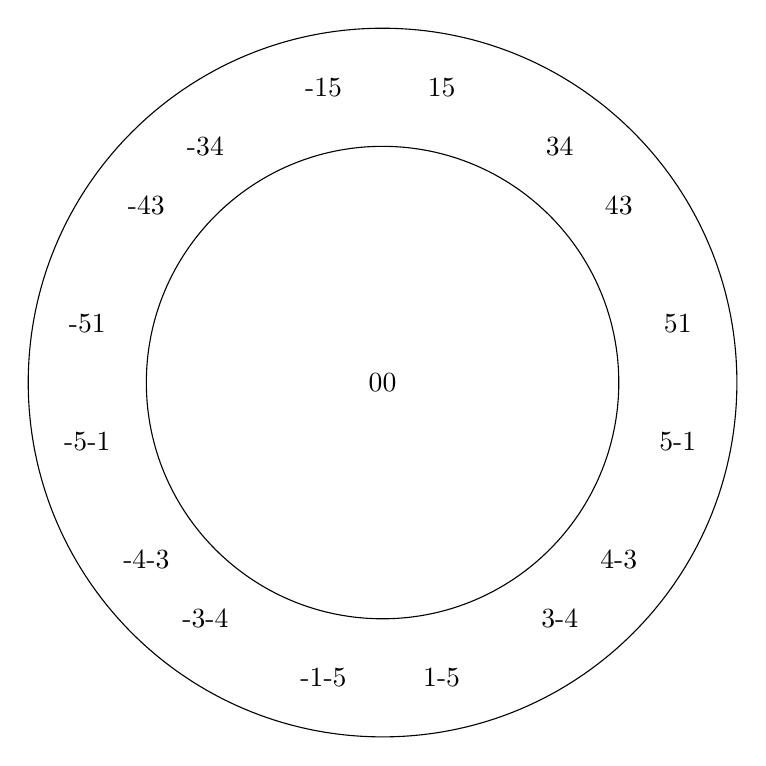
\begin{tikzpicture}[scale=0.75]
	\draw (5,5) circle (4);
	\draw (5,5) circle (6);

	\draw (5, 5) node {\vectwo{0}{0}};

	\draw (4,10) node {\vectwo{-1}{5}};
	\draw (6,10) node {\vectwo{1}{5}};

	\draw (2,9) node {\vectwo{-3}{4}};
	\draw (8,9) node {\vectwo{3}{4}};

	\draw (1,8) node {\vectwo{-4}{3}};
	\draw (9,8) node {\vectwo{4}{3}};

	\draw (0,6) node {\vectwo{-5}{1}};
	\draw (10,6) node {\vectwo{5}{1}};

	\draw (0,4) node {\vectwo{-5}{-1}};
	\draw (10,4) node {\vectwo{5}{-1}};

	\draw (1,2) node {\vectwo{-4}{-3}};
	\draw (9,2) node {\vectwo{4}{-3}};

	\draw (2,1) node {\vectwo{-3}{-4}};
	\draw (8,1) node {\vectwo{3}{-4}};

	\draw (4,0) node {\vectwo{-1}{-5}};
	\draw (6,0) node {\vectwo{1}{-5}};
\end{tikzpicture}
\section{Umsetzung}
\section{Beispiele}